La technologie lighthouse est une technologie de positionnement 3d précis au millimètre près par réception de balayage laser infrarouge initialement conçu pour le HTC Vive.

Elle repose sur le principe d'un phare (lighthouse en anglais) à 2 faisceaux : deux lasers infrarouges diffusés sous forme de plaques balayent la zone de jeu à une fréquence de 60Hz chacun. Les balayages de ces lasers sont déphasés de 180°. Avant chaque balayage, un flash lumineux éclaire la pièce afin de synchroniser les capteurs. Des récepteurs infrarouges placés sur le casque et les manettes permettent de récupérer ces flashs / balayages.

\begin{figure}[ht]
\begin{center}
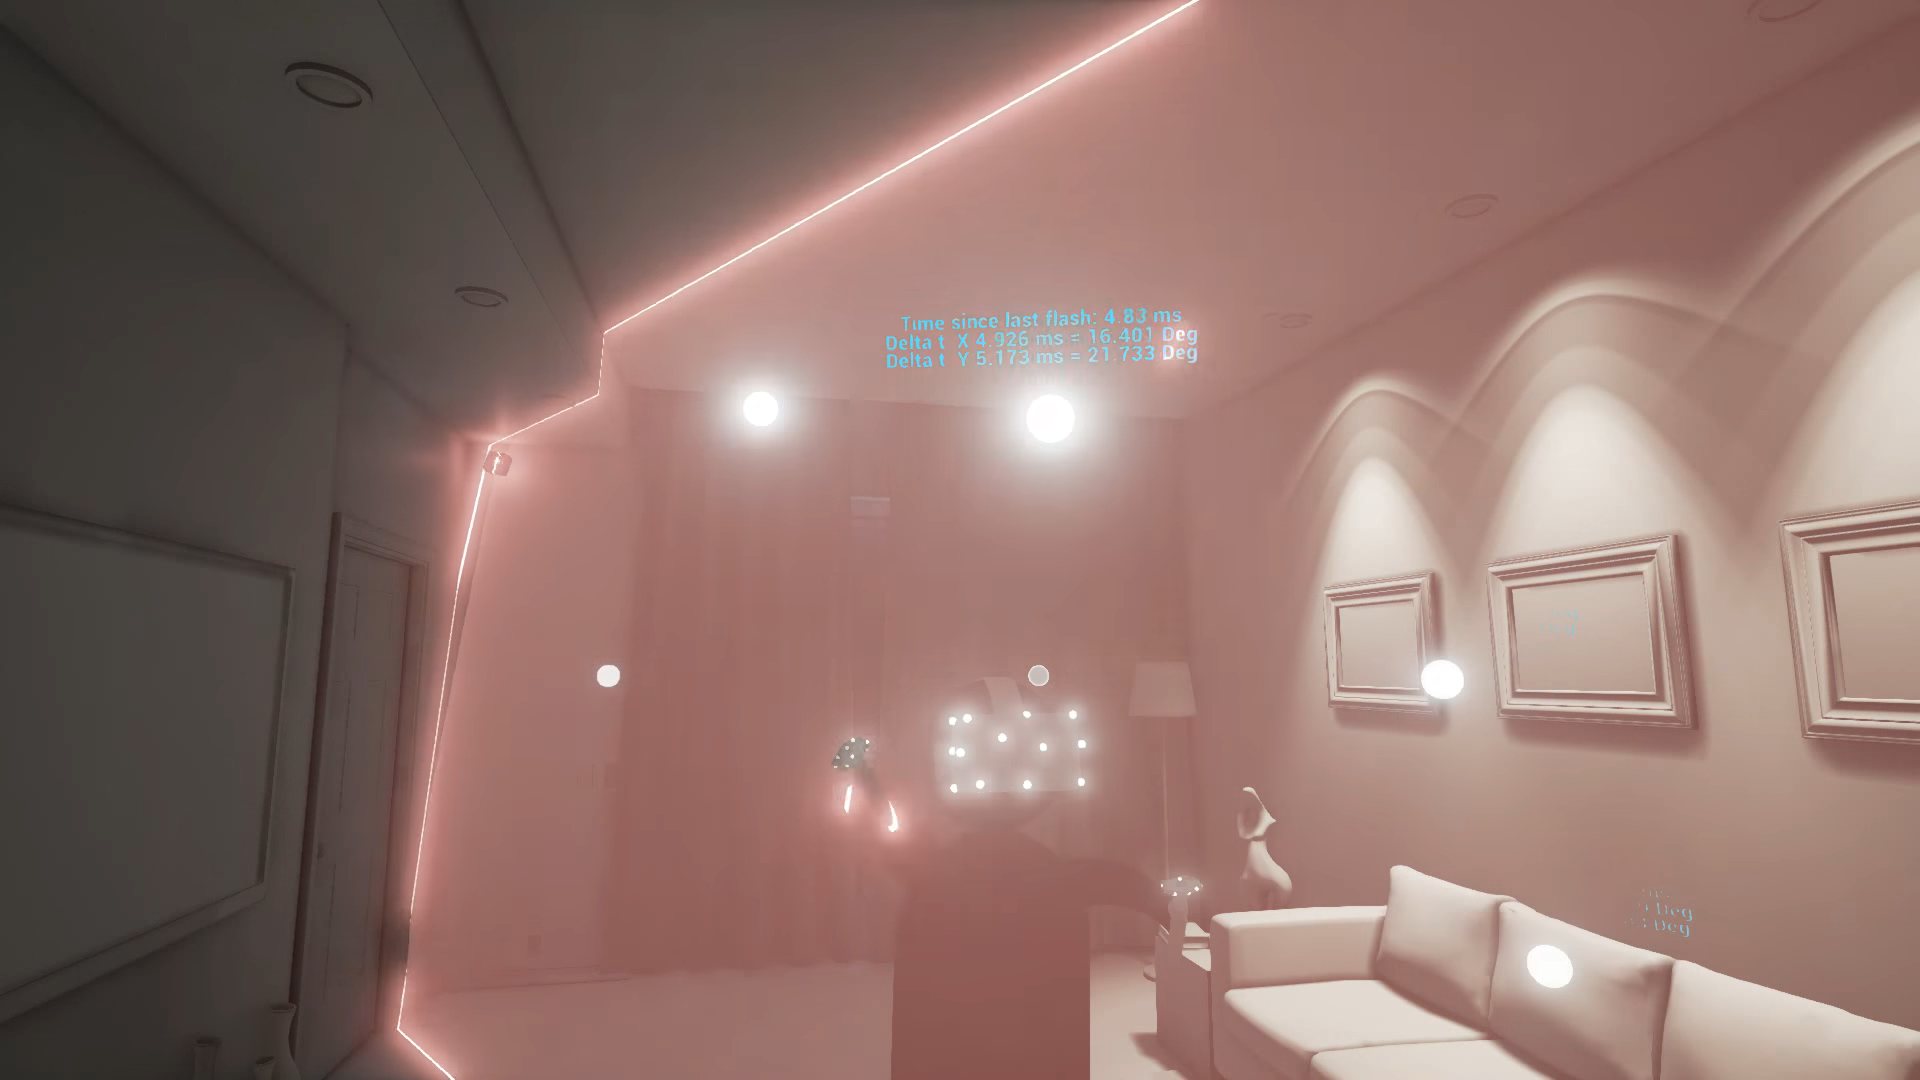
\includegraphics[scale=0.4]{imgs/animation_lighthouse.png}
\end{center}
\caption{Le système "Lighthouse". Cette image est tirée d'une animation disponible sur Youtube à l'adresse : \url{https://www.youtube.com/watch?v=J54dotTt7k0}}
\end{figure}

Sur le HTC Vive, il y a deux "phares" (= balises Lighthouse) placés en hauteur dans deux coins opposés de la zone de jeu, afin de repérer le casque et les manettes en 3D. Elles émettent à tour de rôle. Le cycle complet est alors le suivant :

\begin{figure}[H]
\begin{center}
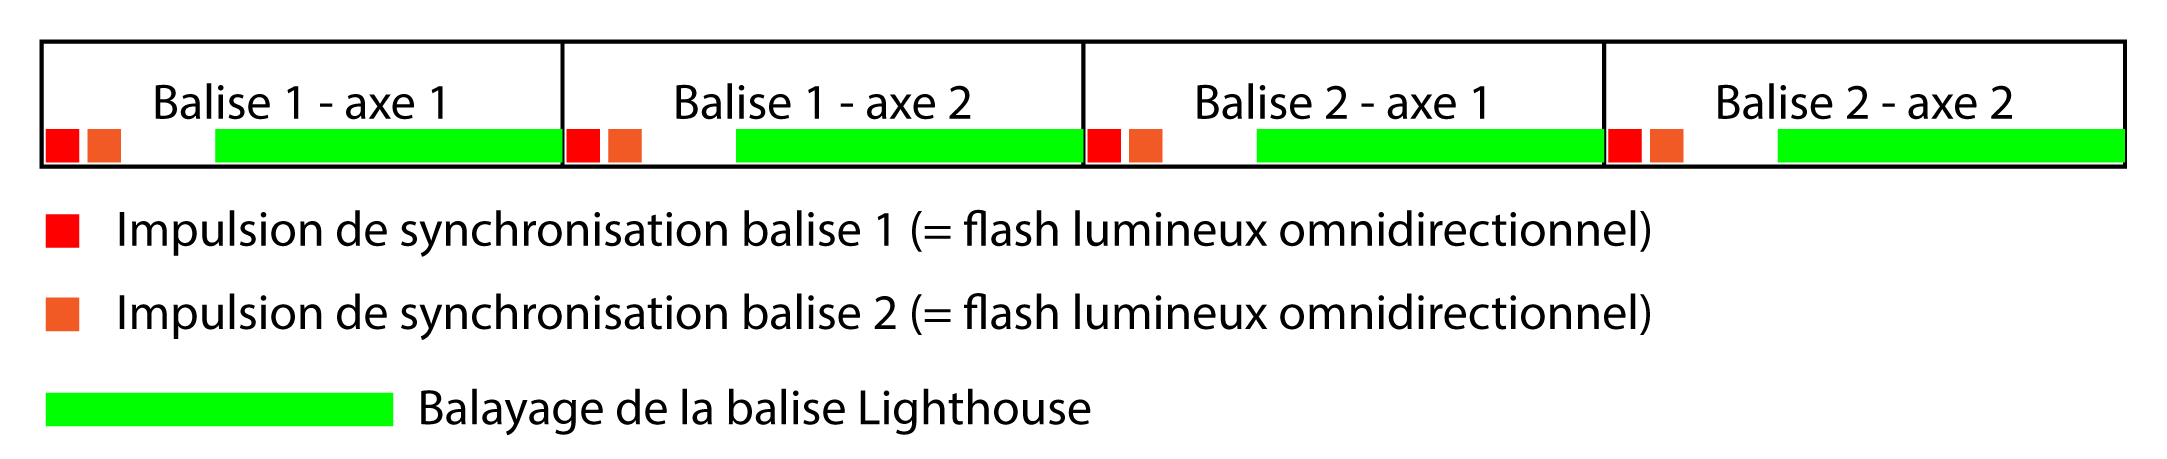
\includegraphics[scale=0.8]{imgs/cycle_balises_lighthouse_deux_balises.png}
\end{center}
\caption{Cycle avec deux balises.}
\end{figure}

Si une seule balise est utilisé, le cycle devient :

\begin{figure}[H]
\begin{center}
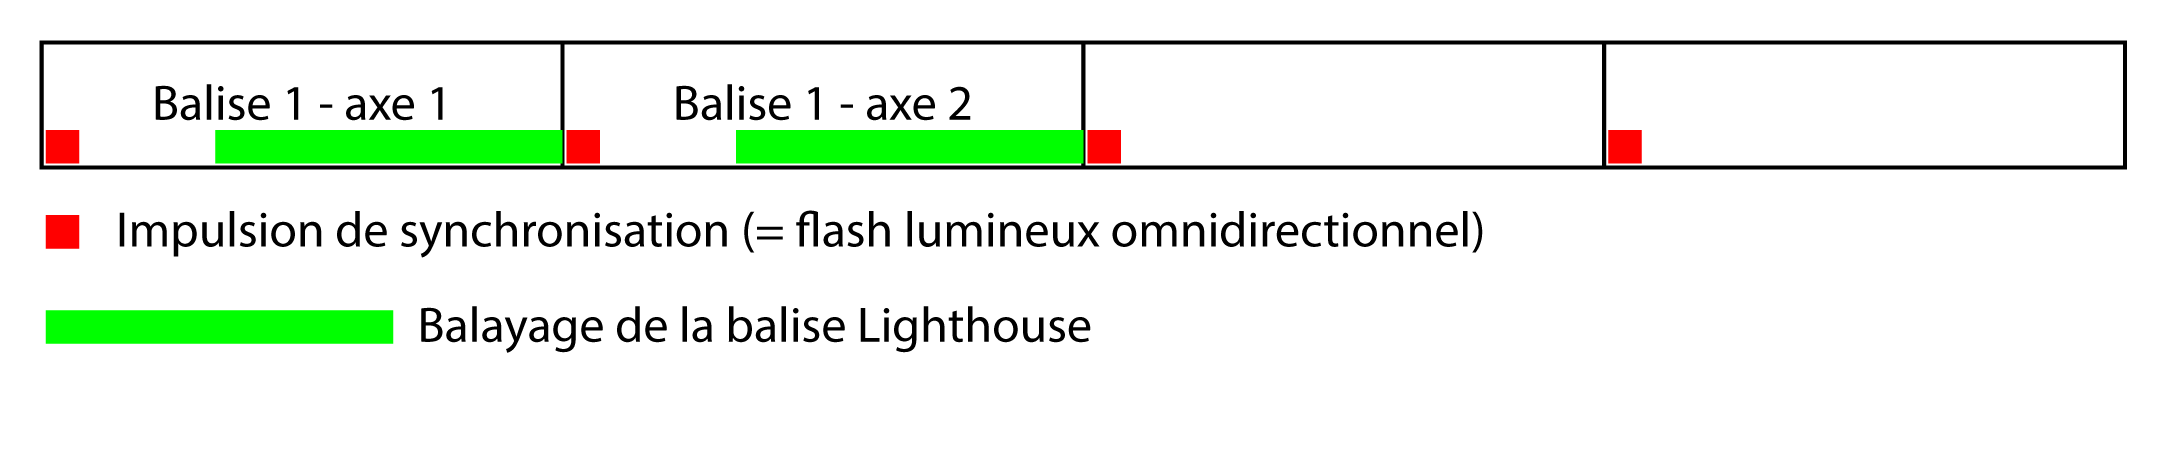
\includegraphics[scale=0.8]{imgs/cycle_balises_lighthouse_une_balise.png}
\end{center}
\caption{Cycle avec une balise.}
\end{figure}

Du point de vue d'un récepteur du HTC Vive, le cycle est :

\begin{figure}[H]
\begin{center}
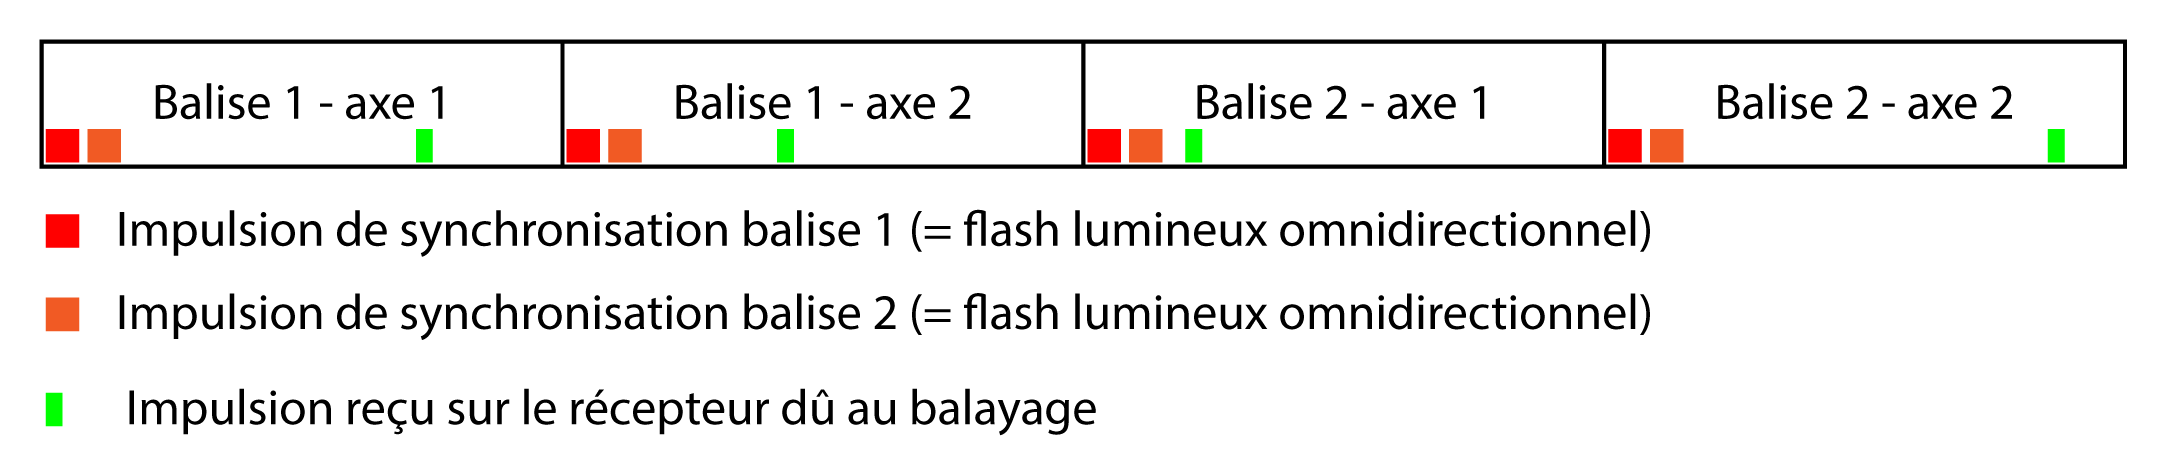
\includegraphics[scale=0.8]{imgs/cycle_balises_lighthouse_deux_balises_recepteur.png}
\end{center}
\caption{Cycle avec deux balises, du point de vue récepteur. La version avec une seule balise est facile à déduire.}
\end{figure}

Le flash est déclenché lorsque le rotor est à son point 0°, ensuite le balayage est effectué à vitesse constante. Le cône d'ouverture au niveau de la balise (= le cône de balayage laser) est de 120°, centré. (60° de part et d'autre de la normale à la vitre d'émission de la balise).